\documentclass[11pt]{article}
\usepackage[a4paper,margin=1.8cm]{geometry}
\usepackage{tikz}
\usepackage{amsmath}
\setcounter{MaxMatrixCols}{10}
\usepackage{amssymb}
\usepackage{xcolor}
\pagestyle{empty}

\begin{document}
\section*{$S=\{0,1,4\}$, $m=3$, $t=5$}
\begin{center}
$\mathbf{FAILURE}$
\end{center}
$\left\lfloor t/2\right\rfloor=2$
\quad\quad
$J=\{1,2\}$
\quad\quad
$N=1$
\quad\quad
$\operatorname{rank}(Y^{+})=1$

\begin{center}
\smallskip Complete graph on $V$, with vertices in $S$ and edges in $E(S)$ highlighted in red. $|E(S)|=3$

\begin{minipage}[t]{0.31\textwidth}
\centering
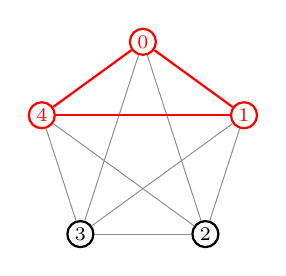
\begin{tikzpicture}[
  thick,
  baseline=(current bounding box.north),
  vertex/.style={circle,draw,inner sep=1.2pt,font=\scriptsize},
  svertex/.style={circle,draw=red,text=red,inner sep=1.2pt,font=\scriptsize}
]
  \node[svertex] (v0) at (0.000,1.350) {0};
  \node[svertex] (v1) at (1.284,0.417) {1};
  \node[vertex] (v2) at (0.794,-1.092) {2};
  \node[vertex] (v3) at (-0.794,-1.092) {3};
  \node[svertex] (v4) at (-1.284,0.417) {4};
  \draw[red] (v0) -- (v1);
  \draw[black!45,line width=0.35pt] (v0) -- (v2);
  \draw[black!45,line width=0.35pt] (v0) -- (v3);
  \draw[red] (v0) -- (v4);
  \draw[black!45,line width=0.35pt] (v1) -- (v2);
  \draw[black!45,line width=0.35pt] (v1) -- (v3);
  \draw[red] (v1) -- (v4);
  \draw[black!45,line width=0.35pt] (v2) -- (v3);
  \draw[black!45,line width=0.35pt] (v2) -- (v4);
  \draw[black!45,line width=0.35pt] (v3) -- (v4);
\end{tikzpicture}
\end{minipage}
\par\smallskip Jumps in $E(S)$: $J=\{1,2\}$
\par $b_{01} + b_{04} + b_{14} \le d_m(|S|)=d_{3}(3)=2$
\par $2 y_{1} + y_{2} \le 2$
\end{center}

Each drawing below is a circulant graph $G_{L}$ for a non-empty $L\subseteq J$ with edges $E(L)=\{\{i,j\}\mid i,j\in V,\ \min((i-j)\bmod t,\,(j-i)\bmod t)\in L\}$.
For each graph, we show $|E(L)\cap E(S)|$ and put $\textcolor{green!60!black}{\checkmark}$ iff $|E(L)\cap E(S)|=d_m(|S|)$; otherwise $\textcolor{red}{\boldsymbol{\times}}$.
All non-empty jump sets are shown.

\noindent
\begin{minipage}[t]{0.31\textwidth}
\centering
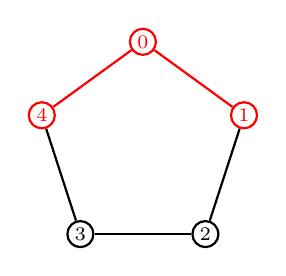
\begin{tikzpicture}[
  thick,  vertex/.style={circle,draw,inner sep=1.2pt,font=\scriptsize},  svertex/.style={circle,draw=red,text=red,inner sep=1.2pt,font=\scriptsize},  baseline=(current bounding box.north)
]
  \node[svertex] (v0) at (0.000,1.350) {0};
  \node[svertex] (v1) at (1.284,0.417) {1};
  \node[vertex] (v2) at (0.794,-1.092) {2};
  \node[vertex] (v3) at (-0.794,-1.092) {3};
  \node[svertex] (v4) at (-1.284,0.417) {4};
  \draw[red] (v0) -- (v1);
  \draw[red] (v0) -- (v4);
  \draw (v1) -- (v2);
  \draw (v2) -- (v3);
  \draw (v3) -- (v4);
\end{tikzpicture}
\par\smallskip Graph 1
\par $L=\{\textcolor{red}{1}\}$
\par $y=\left(\textcolor{red}{1},\textcolor{red}{0}\right)$
\par $|E(L)\cap E(S)|=2\;\;\textcolor{green!60!black}{\checkmark}$
\end{minipage}\hfill\begin{minipage}[t]{0.31\textwidth}
\centering
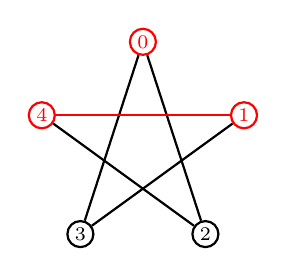
\begin{tikzpicture}[
  thick,  vertex/.style={circle,draw,inner sep=1.2pt,font=\scriptsize},  svertex/.style={circle,draw=red,text=red,inner sep=1.2pt,font=\scriptsize},  baseline=(current bounding box.north)
]
  \node[svertex] (v0) at (0.000,1.350) {0};
  \node[svertex] (v1) at (1.284,0.417) {1};
  \node[vertex] (v2) at (0.794,-1.092) {2};
  \node[vertex] (v3) at (-0.794,-1.092) {3};
  \node[svertex] (v4) at (-1.284,0.417) {4};
  \draw (v0) -- (v2);
  \draw (v0) -- (v3);
  \draw (v1) -- (v3);
  \draw[red] (v1) -- (v4);
  \draw (v2) -- (v4);
\end{tikzpicture}
\par\smallskip Graph 2
\par $L=\{\textcolor{red}{2}\}$
\par $y=\left(\textcolor{red}{0},\textcolor{red}{1}\right)$
\par $|E(L)\cap E(S)|=1\;\;\textcolor{red}{\boldsymbol{\times}}$
\end{minipage}\hfill\begin{minipage}[t]{0.31\textwidth}
\centering
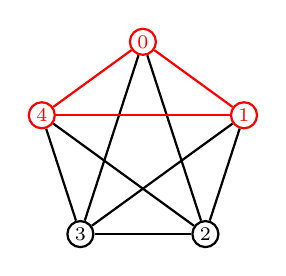
\begin{tikzpicture}[
  thick,  vertex/.style={circle,draw,inner sep=1.2pt,font=\scriptsize},  svertex/.style={circle,draw=red,text=red,inner sep=1.2pt,font=\scriptsize},  baseline=(current bounding box.north)
]
  \node[svertex] (v0) at (0.000,1.350) {0};
  \node[svertex] (v1) at (1.284,0.417) {1};
  \node[vertex] (v2) at (0.794,-1.092) {2};
  \node[vertex] (v3) at (-0.794,-1.092) {3};
  \node[svertex] (v4) at (-1.284,0.417) {4};
  \draw[red] (v0) -- (v1);
  \draw (v0) -- (v2);
  \draw (v0) -- (v3);
  \draw[red] (v0) -- (v4);
  \draw (v1) -- (v2);
  \draw (v1) -- (v3);
  \draw[red] (v1) -- (v4);
  \draw (v2) -- (v3);
  \draw (v2) -- (v4);
  \draw (v3) -- (v4);
\end{tikzpicture}
\par\smallskip Graph 3
\par $L=\{\textcolor{red}{1},\textcolor{red}{2}\}$
\par $y=\left(\textcolor{red}{1},\textcolor{red}{1}\right)$
\par $|E(L)\cap E(S)|=3\;\;\textcolor{red}{\boldsymbol{\times}}$
\end{minipage}
\par\medskip

\noindent\textbf{Matrix Data}
\par $N=1$
\par $I=\{1\}$\quad$Y=\begin{bmatrix}1 \\ 0\end{bmatrix}$
\par $Y^{+}=\begin{bmatrix}1 \\ 0 \\ 1\end{bmatrix}$\quad$\operatorname{rank}(Y^{+})=1$
\end{document}
